
\subsection{Analysis of Optimal Number of ICs} \label{sec:optimal}

After having undergone the initial standard preprocessing presented in \secref{sec:std}, the next step was to extract the ICs using MELODIC. But before the data could be subjected to the ICA, several considerations were made in order to increase ICA performance. The separation of sources is highly dependent on the number of ICs (n-ICs) chosen and therefore crucial for the FIX end performance. Consequently, an investigation of the optimal number of components was conducted. The risk of underestimating the number of components, would result in a loss of information and suboptimal signal extraction \cite{Beckmann2004}. Contrarily, overestimating the number of components would result in a false representation, as the different informative sources would be split leaving sources fragmented, which would be hard to identify and utilize \cite{Beckmann2004,Li2007}. \\
Data used for investigating the optimal number of components was derived from ten randomly chosen participants having three heat runs each. 
%This made for 30 IC analyses each completed utilizing the MELODIC tool. 


\subsubsection{Default setting}
Initially no limit was selected and the MELODIC algorithm per default estimated the optimal number of components. \cite{FMRIB2016} The MELODIC tool provided analyses with the automatically estimated number of components to represent the variance ranging from 9 to 64 components per heat run. Due to the substantial amount of variability in the number of components estimated, the degree to how much the sources had been separated varied substantially between the scans. Inspecting the output from the ICA, which only estimated nine components, it became clear that the separation of sources was not sufficient, as the components were mixtures of multiple sources of noise and signal. Furthermore, sparse non-localized task-related activation was seen in any of the components indicating that variance of noise accounted for the first nine components. Qualitatively inspecting the analyses with the highest number of components, it became evident that the algorithm had overestimated the number of ICs, leaving empty and fragmented activation in the components, which could not be identified and thus properly labeled. It was assessed that using MELODIC with default setting would be overestimating and underestimating the number of components. Therefore, a case specific analysis for the optimal number of components was conducted. 

\subsubsection{n-IC analysis}

Seeking guidelines in the literature, various articles have worked with estimating the optimal number of components. In the case of Majeed et al. \cite{Majeed2014}, results indicate that a n-IC lower than 5 components would lead to an underestimation and more than 50 components would result in overestimation. In this case the optimal n-IC was found to be 10. Another study limited the number of components to 20, as this was found to preserve much of the information without overestimating \cite{Calhoun2001}. Furthermore other studies limited the number to 25 components \cite{Kim2013,Erpelding2013}. Building on this knowledge, MELODIC was run on the 30 heats runs limiting the n-ICs to 15, 20, 25, 30 in order to assess which n-IC would give the optimal separation between signal and noise, and subsequently separation of each source. The qualitative assessment was made by counting the following outcomes: 
\begin{itemize}
	\item The number of components containing activation from multiple sources or being unrecognizable 
	\item The number of components containing activation from a single source 
	\item The number of components containing no activation    
\end{itemize}
 
Examples of spatial maps (inferior to superior) containing multiple sources, fragmented sources and a single source can be seen in \figref{fig:meth:Unknown_mix}, \figref{fig:meth:Frag} and \figref{fig:meth:Move}, respectively. Identification of sources was supported by utilizing the guidelines presented in \cite{Griffanti2017}, which illustrated how the different noise sources appeared in the spatial map, along with the information of which brain regions would be activated during noxious stimuli as presented in \secref{sec:pain}. Both investigators conducted the assessment. One found 25 components to be optimal, whilst the other found that 30 components was more favorable. The assessment was assisted by incorporating an expert's opinion. Integrating the expert's opinion, 25 components was assessed to provide the best separation of sources in the data. This decision was supported by the results of the prior studies of \cite{Kim2013,Erpelding2013}.     

\begin{figure}[H]                 
	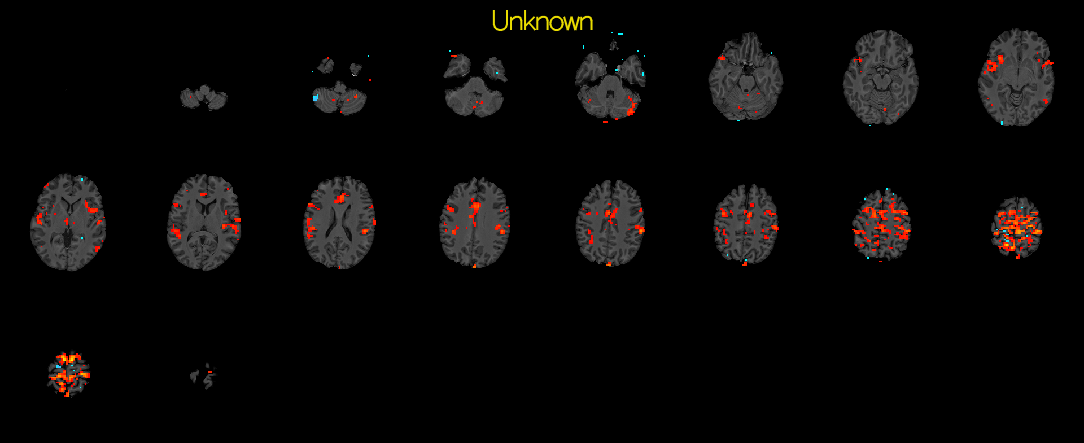
\includegraphics[width=.85\textwidth]{figures/bMethods/Unknown_mix}  
	\caption{An example of a  component with a spatial map for a component showing activation from multiple sources. Activation could not be localized to single brain regions, and was a mixture of noise and signal.}
	\label{fig:meth:Unknown_mix} 
\end{figure}

\begin{figure}[H]                 
	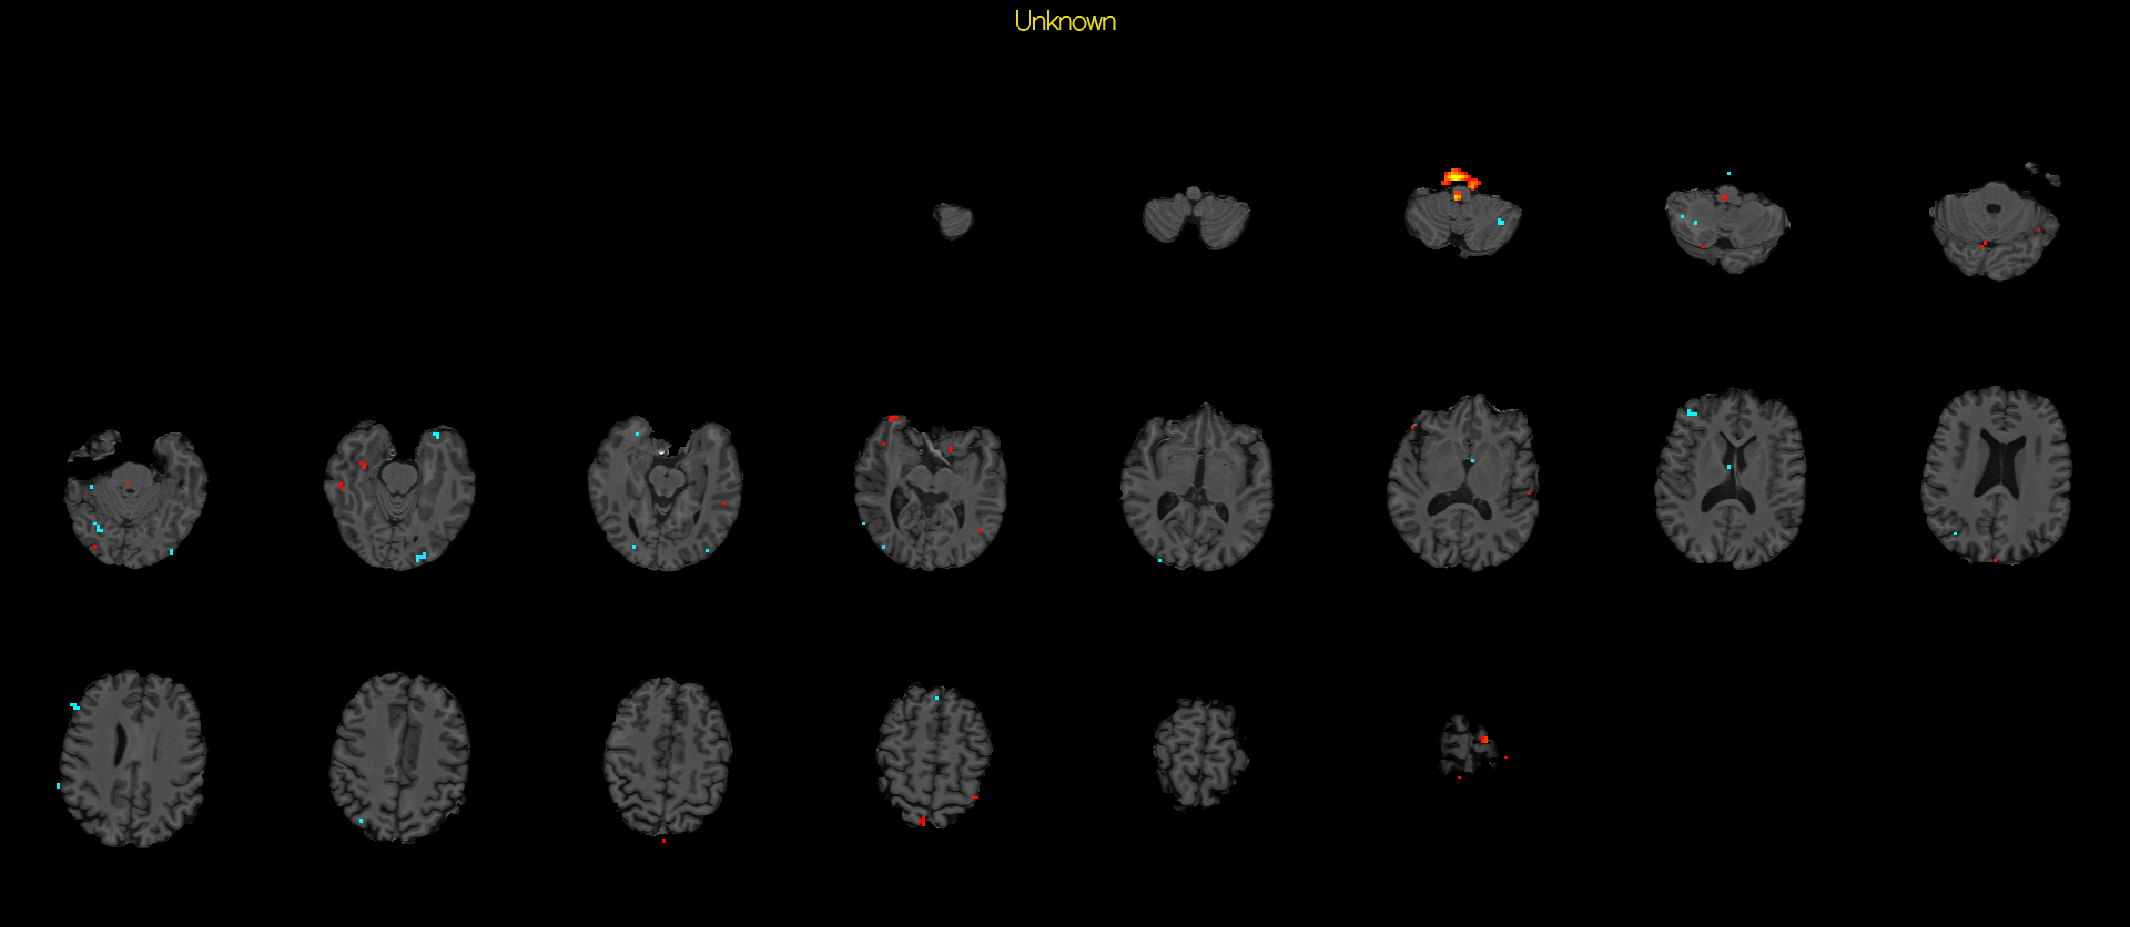
\includegraphics[width=.85\textwidth]{figures/bMethods/Frag}  
	\caption{An example of a component with a fragmented spatial map illustrating that no brain activation or noise can be localized.}
	\label{fig:meth:Frag} 
\end{figure}

\begin{figure}[H]                 
	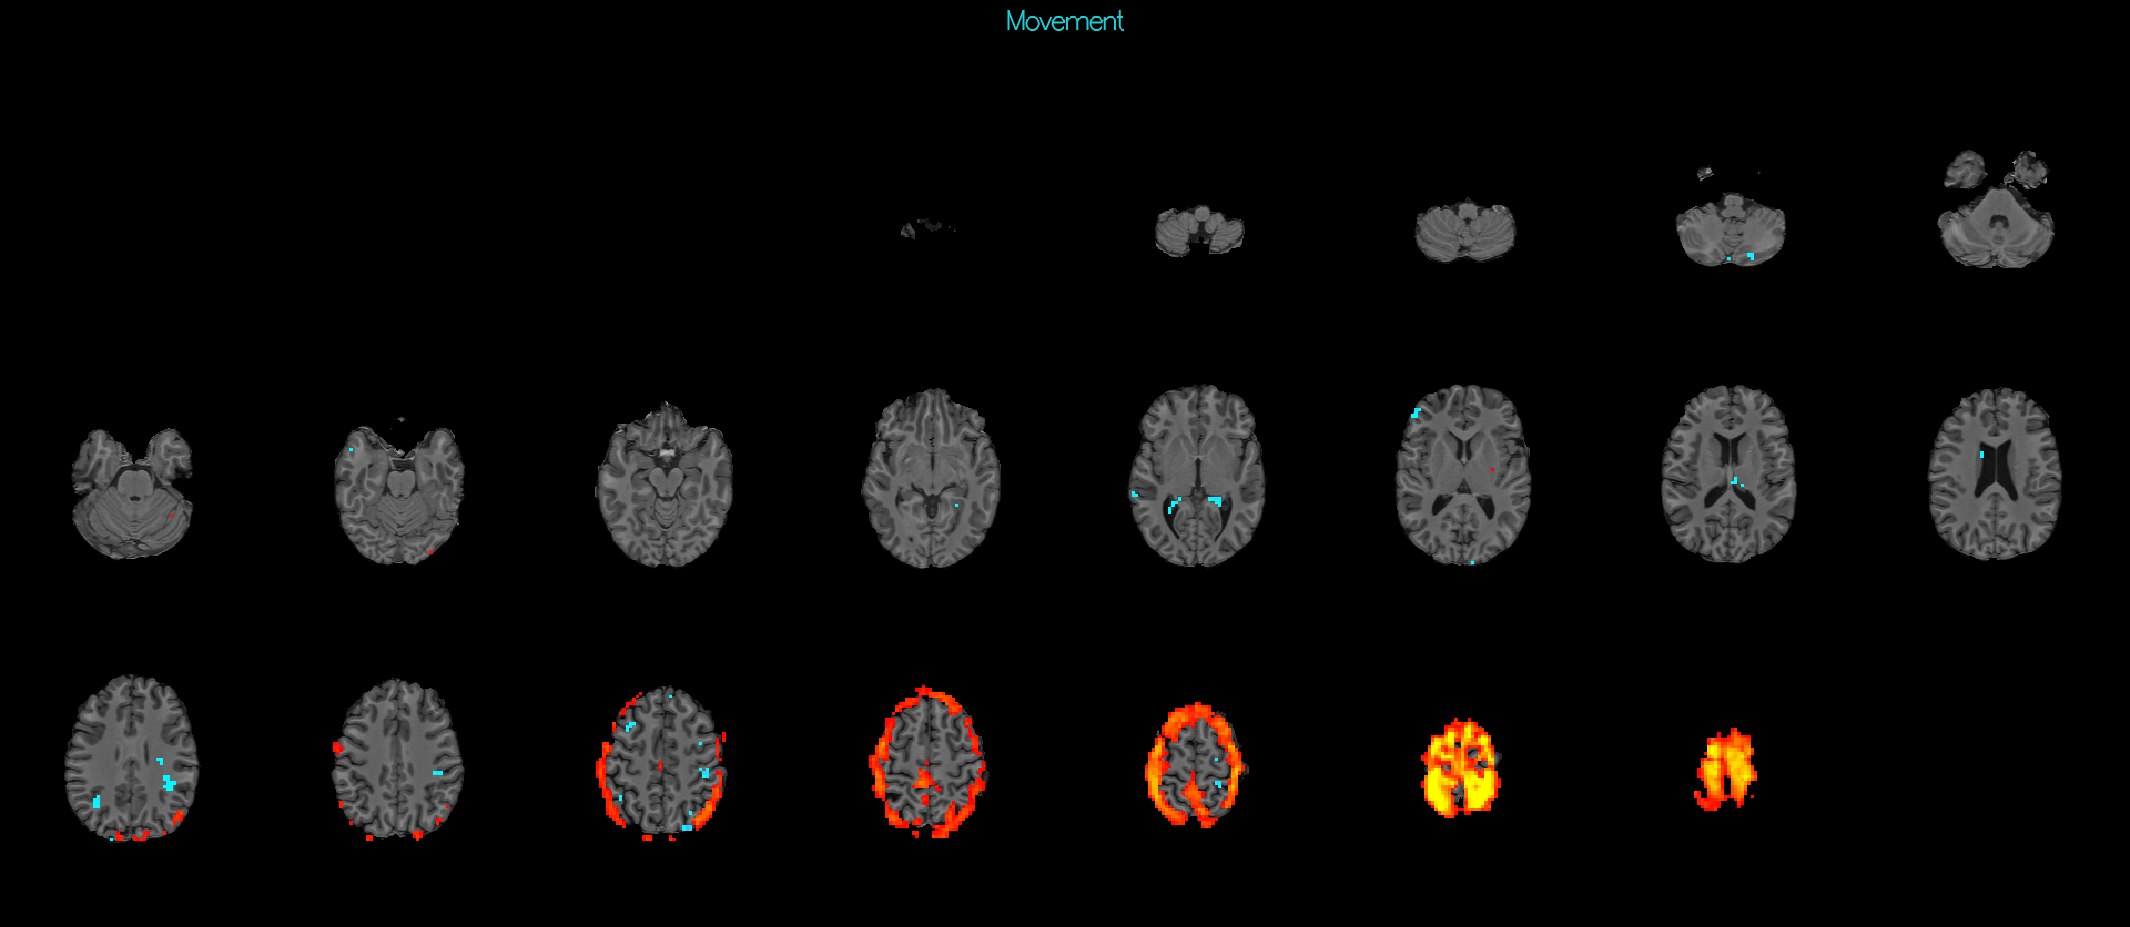
\includegraphics[width=.85\textwidth]{figures/bMethods/Movement}  
	\caption{An example of a spatial map showing a clearly recognizable single source artifact in the form of movement dominating the component.}
	\label{fig:meth:Move} 
\end{figure}






 